\documentclass{ctexart}

% --- 导入所需宏包 ---
\usepackage[a4paper, vmargin=2.5cm, hmargin=2cm]{geometry}
\usepackage{amsmath, amssymb, amsthm}
\usepackage[svgnames]{xcolor}
\usepackage[most]{tcolorbox}
\usepackage{fancyhdr}
\usepackage{tikz}
\usetikzlibrary{intersections, patterns, shadows, decorations.pathmorphing}
\usepackage{fontawesome5} % 更新的图标包
\usepackage{enumitem}
\usepackage{mdframed}

% --- 自定义优雅颜色定义 ---
\definecolor{themeblue}{RGB}{52, 73, 94}
\definecolor{elegantpurple}{RGB}{155, 89, 182}
\definecolor{warmorange}{RGB}{230, 126, 34}
\definecolor{forestgreen}{RGB}{39, 174, 96}
\definecolor{deepblue}{RGB}{41, 128, 185}
\definecolor{sunsityellow}{RGB}{241, 196, 15}
\definecolor{lightgrayblue}{RGB}{236, 240, 241}
\definecolor{softpink}{RGB}{250, 219, 216}

% --- 页面布局与页眉页脚设置 ---
\pagestyle{fancy}
\fancyhf{}
\fancyhead[L]{\color{themeblue}\textbf{\faBook\ 解析几何}}
\fancyhead[R]{\color{themeblue}\textit{听尽江南雨 \faUser}}
\fancyfoot[C]{\color{themeblue!70}\small\textbf{--\ \thepage\ --}}
\renewcommand{\headrulewidth}{1pt}
\renewcommand{\footrulewidth}{0pt}
\renewcommand{\headrule}{\hbox to\headwidth{\color{themeblue!30}\leaders\hrule height \headrulewidth\hfill}}

% --- 自定义优美的文本框环境 ---

% 习题框 (专业方正设计,左侧竖线,优化对齐)
\newtcolorbox{exercisebox}[1]{
    enhanced,
    colback=white,
    colframe=white,
    boxrule=0pt,
    arc=0pt,
    outer arc=0pt,
    fonttitle=\sffamily\bfseries\Large,
    title={\makebox[1.5em][l]{\textcolor{forestgreen}{\faEdit}}\ \textit{Exercise} #1 \quad 习题},
    coltitle=forestgreen,
    colbacktitle=white,
    attach boxed title to top left={yshift=0mm, xshift=0mm},
    boxed title style={arc=0pt, outer arc=0pt, frame hidden},
    borderline west={4pt}{0pt}{forestgreen},
    left=15pt, right=10pt, top=15pt, bottom=10pt,
    before skip=20pt, after skip=15pt,
    breakable
}

% 解析框 (专业方正设计,左侧竖线,优化对齐)
\newtcolorbox{analysisbox}{
    enhanced,
    colback=elegantpurple!5!white,
    colframe=white,
    boxrule=0pt,
    arc=0pt,
    outer arc=0pt,
    fonttitle=\sffamily\bfseries\Large,
    title={\makebox[1.5em][l]{\textcolor{elegantpurple}{\faLightbulb}}\ \textit{Analysis} \quad 解析思路},
    coltitle=elegantpurple,
    colbacktitle=elegantpurple!5!white,
    attach boxed title to top left={yshift=0mm, xshift=0mm},
    boxed title style={arc=0pt, outer arc=0pt, frame hidden},
    borderline west={4pt}{0pt}{elegantpurple},
    left=15pt, right=10pt, top=15pt, bottom=10pt,
    before skip=20pt, after skip=15pt,
    breakable
}

% 拓展框 (专业方正设计,左侧竖线,优化对齐)
\newtcolorbox{expandbox}{
    enhanced,
    colback=warmorange!8!white,
    colframe=white,
    boxrule=0pt,
    arc=0pt,
    outer arc=0pt,
    fonttitle=\sffamily\bfseries\Large,
    title={\makebox[1.5em][l]{\textcolor{warmorange}{\faRocket}}\ \textit{Extension} \quad 知识拓展},
    coltitle=warmorange,
    colbacktitle=warmorange!8!white,
    attach boxed title to top left={yshift=0mm, xshift=0mm},
    boxed title style={arc=0pt, outer arc=0pt, frame hidden},
    borderline west={4pt}{0pt}{warmorange},
    left=15pt, right=10pt, top=15pt, bottom=10pt,
    before skip=20pt, after skip=15pt,
    breakable
}

% --- 数学公式和排版优化 ---
\renewcommand{\arraystretch}{1.4}
\setlength{\jot}{8pt}

% 自定义数学命令
\newcommand{\highlight}[1]{\colorbox{sunsityellow!20}{\ensuremath{#1}}}
\newcommand{\result}[1]{\tcbhighmath[colback=deepblue!15, colframe=deepblue, arc=3pt]{#1}}

% --- 文档开始 ---
\begin{document}
\thispagestyle{fancy}

% 优美的章节标题 (主标题斜体英文+中文)
\begin{center}
    \begin{tcolorbox}[
        enhanced,
        colback=themeblue!8!white,
        colframe=white,
        boxrule=0pt,
        arc=0pt,
        width=0.90\textwidth,
        fonttitle=\Huge\sffamily\bfseries,
        title={\makebox[1.5em][l]{\textcolor{themeblue}{\faCalculator}}\ \textit{\Large{Miquel's Theorem 4.36}} \quad 米勒定理},
        coltitle=themeblue,
        center title,
        toptitle=15pt,
        bottomtitle=15pt,
        borderline west={5pt}{0pt}{themeblue}
    ]
    \vspace{8pt}
    \end{tcolorbox}
\end{center}

\vspace{15pt}

\begin{exercisebox}{127}
已知 $A(-1, 0)$,$B(3, 0)$。$P$ 是圆 $O: x^2+y^2=36$ 上的一个动点,则 $\sin \angle APB$ 的最大值为:\underline{\hspace{4cm}}。
\end{exercisebox}

\begin{analysisbox}
\textbf{\color{elegantpurple}\textit{Solution Strategy} \quad 解题思路:}

\begin{enumerate}[leftmargin=15pt, itemsep=8pt]
    \item 考虑圆的对称性,仅研究上半圆。取点 $P$,使 $\triangle ABP$ 的外接圆与动圆 $O$ 相切于点 $P$。
    
    \item 另取一点 $P_1$,则易见 $\angle APB > \angle AP_1 B$。故 $\triangle ABP$ 的外接圆 $E$ 与圆 $O$ 相切时,有最大的 $\angle APB$。
    
    \item 考虑 $0 < \angle APB < \frac{\pi}{2}$,即此时有最大的 $\sin \angle APB$。
\end{enumerate}

\medskip
\textbf{\color{elegantpurple}\textit{Detailed Calculation} \quad 具体计算:}

设外接圆圆心 $E(1, t)$,则其半径 $R_{E} = EB$。

根据两圆内切条件,圆心距等于半径差,即 $\highlight{OE = R_O - R_E}$。

\begin{align}
R_E &= \sqrt{(3-1)^2+t^2} = \sqrt{4+t^2} \\
OE &= \sqrt{(1-0)^2+t^2} = \sqrt{1+t^2} \\
R_O &= 6
\end{align}

代入得 $\sqrt{4+t^2} = 6 - \sqrt{1+t^2}$,解得 $\sqrt{4+t^2} = \frac{13}{4}$。

\medskip
\textbf{\color{elegantpurple}\textit{Final Answer} \quad 最终答案:}

根据正弦定理:
\result{\sin\angle APB = \frac{AB}{2R_E} = \frac{4}{2 \times \frac{13}{4}} = \frac{8}{13}}
\end{analysisbox}

\begin{figure}[h!]
\centering
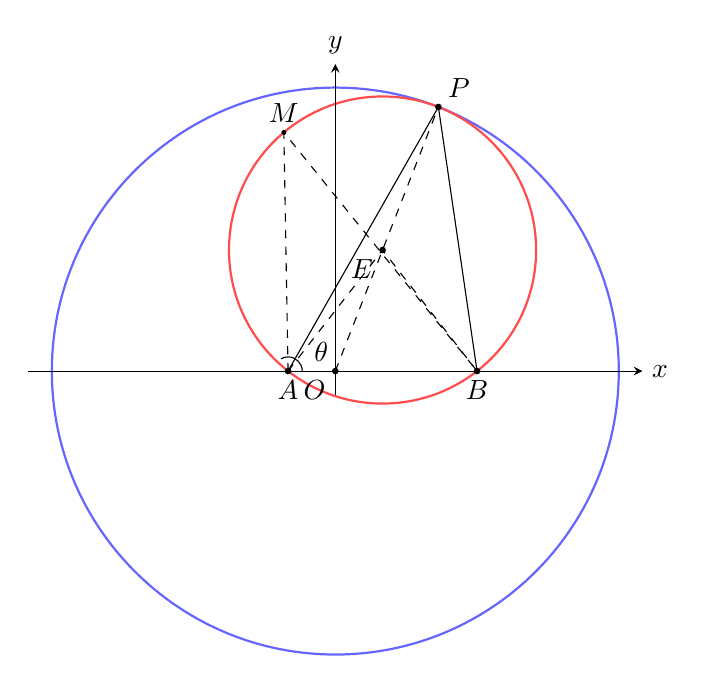
\begin{tikzpicture}[scale=0.6, >=stealth]
    % 定义坐标
    \coordinate (O) at (0,0); % 大圆圆心 (原点)
    \coordinate (A) at (-1,0);
    \coordinate (B) at (3,0);
    
    % 计算外接圆圆心 E 和切点 P
    % R_E = 13/4, OE = 11/4, t = sqrt(105)/4
    \pgfmathsetmacro{\t}{sqrt(105)/4}
    \pgfmathsetmacro{\RE}{13/4}
    \pgfmathsetmacro{\OE}{11/4}
    \coordinate (E) at (1, {\t});
    
    % P 是 O, E 连线的延长线与大圆的交点
    % P = (6/OE) * E
    \coordinate (P) at ({6/\OE}, {6/\OE * \t});
    
    % 绘制大圆O
    \draw[name path=circleO, thick, blue!60] (O) circle (6);
    
    % 绘制三角形APB的外接圆
    \draw[name path=circleE, thick, red!70] (E) circle (\RE);
    
    % 绘制坐标轴和辅助线
    \draw[->] (-6.5,0) -- (6.5,0) node[right] {$x$};
    \draw[->] (0,-0.5) -- (0,6.5) node[above] {$y$};
    \draw[dashed] (O) -- (P);
    \draw[dashed] (A) -- (E);
    \draw[dashed] (B) -- (E);

    % 绘制三角形和弦
    \draw (A) -- (P) -- (B);
    
    % 标记点
    \fill (O) circle (2pt) node[below left] {$O$};
    \fill (A) circle (2pt) node[below] {$A$};
    \fill (B) circle (2pt) node[below] {$B$};
    \fill (P) circle (2pt) node[above right] {$P$};
    \fill (E) circle (2pt) node[below left] {$E$};
    
    % 虚构一个M点
    \coordinate (M) at ({-13/4 * cos(50) + 1}, {\RE * sin(50) + \t});
    \draw[dashed] (A) -- (M) -- (B);
    \fill (M) circle (1.5pt) node[above] {$M$};
    
    % 添加角度标记
    \draw (A) ++(0.3,0) arc (0:120:0.3);
    \node at (-0.3, 0.4) {$\theta$};

\end{tikzpicture}
\caption{\textcolor{themeblue}{\textbf{\textit{Figure 4.49 - Miquel's Theorem Geometry} \quad 图 4.49 - 米勒定理几何示意图}}}
\label{fig:miquel}
\end{figure}

\begin{expandbox}
该题为米勒定理的变式,最大临界角的证明,依然采用了圆周角大于圆外角的方式。具体问题的原型为 $\angle MON$ 一边 $ON$ 上有定点 $A,B$,另一边 $OM$ 上有动点 $P$,求 $\angle APB$ 何时最大。
不难证明 $\triangle APB$ 的外接圆与 $OM$ 相切于点 $P$。证明方式与本题一致,都是另取一点,利用圆周角大于圆外角处理。
\end{expandbox}

\newpage
\setcounter{page}{147}

\end{document}